% Capacity and demand per bolt, log scale.
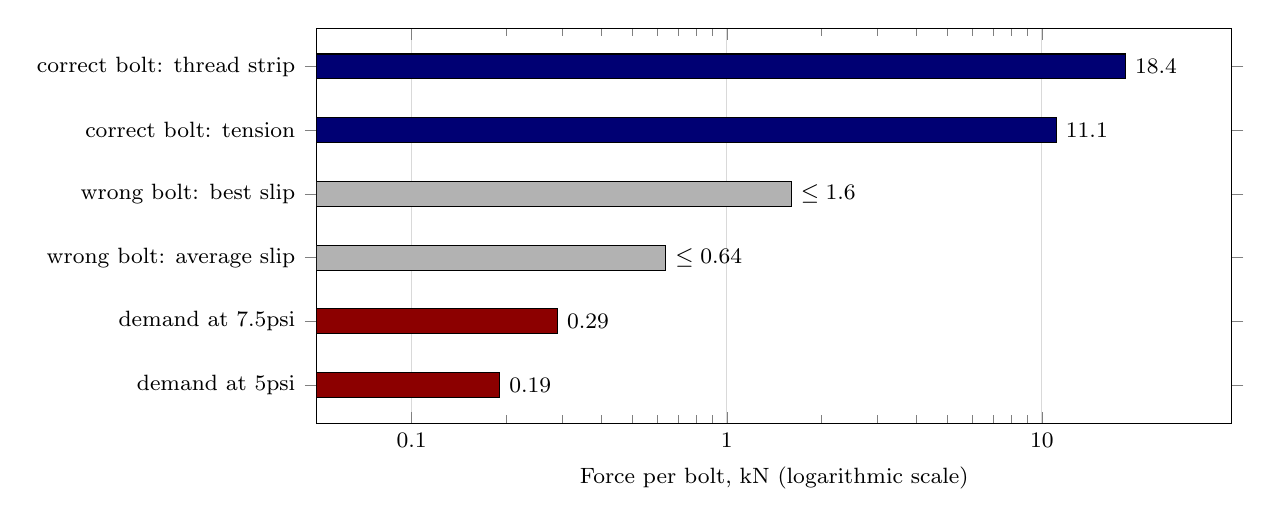
\begin{tikzpicture}
\begin{axis}[xbar,xmode=log,log origin=infty,width=13.2cm,height=6.6cm,xmin=0.05,xmax=40,
  bar width=9pt,bar shift=0pt,enlarge y limits=0.12,
  xlabel={Force per bolt, kN (logarithmic scale)},
  ytick={1,2,3,4,5,6},
  yticklabels={{demand at \SI{5}{psi}},{demand at \SI{7.5}{psi}},{wrong bolt: average slip},{wrong bolt: best slip},{correct bolt: tension},{correct bolt: thread strip}},
  yticklabel style={font=\footnotesize,align=right},xticklabel style={font=\footnotesize},xlabel style={font=\footnotesize},
  xtick={0.1,1,10},xticklabels={0.1,1,10},
  nodes near coords,nodes near coords style={font=\footnotesize,anchor=west},point meta=explicit symbolic,
  xmajorgrids,grid style={black!15}]
\addplot[fill=red!55!black,draw=black] coordinates {(0.19,1)[0.19] (0.29,2)[0.29]};
\addplot[fill=black!30,draw=black] coordinates {(0.64,3)[$\le0.64$] (1.6,4)[$\le1.6$]};
\addplot[fill=blue!45!black,draw=black] coordinates {(11.1,5)[11.1] (18.4,6)[18.4]};
\end{axis}
\end{tikzpicture}
